\documentclass{ltjsbook}
\usepackage{docmute} 
\usepackage{../../myStyle} 

\begin{document}
\VerbatimFootnotes
\chapter{記述統計量}
\label{ch05_descriptives}

さて，ここまでで心理学においてなぜ統計学が必要か，計算機とはどういうものか，計算機に与えるデータはどういうものか，という話をしてきました。下準備はそこまでです。いよいよ，今回から心理統計の具体的な話に入っていきます。

初めに，心理統計の3つの枠組みを紹介しておきます。
\begin{description}
	\item[記述統計 descriptive statistics] データの特徴を記述する統計法。可視化，代表値による要約など。 データを取ったらまずやるべき作業がこちら。手元のデータでわかることを，隅々まで書き表すのが狙いです。
	\item[推測統計 inferential statistics] 部分的なデータから全体像を推測する統計学。心理統計の目的は一部のサンプルから全体を予測することにあるのです。この授業の後半(後期)は主にこの話になります。
	\item[多変量解析 multivariate analysis] 大量のデータから意味のある情報を引き出す，あるいは無意味な情報を削ぎ落とす技術です。調査研究をする場合はもちろん，センサーなどの機器から大量に取れるデータを扱う場合にも使われる技術です。データサイエンス，機械学習(いわゆるAI)などにも通じる領域です。本学では2年のデータ解析応用で扱います。
\end{description}

ということで，ここにあるように記述統計学が最初のステップになります。手元にあるデータの特徴を記述することが目的になります。記述という意味では可視化もそうなのですが，今回は数字によってデータの特徴を記述することを考えます。複数のデータの代表的な値ですから，代表値と言われたりします。

研究対象を数値化したとしましょう。それを眺めて「いろいろな数字があるなあ」と感心していたのでは，数値化した意味がありません。得られた\textbf{データは図にする}のが基本です。すぐに図にします。いろいろな図にします。前回も話しましたが，とにかく図にします。しなければなりません。さて，図を見て考えをまとめるのが重要なのですが，具体的にどういう特徴があるのか，あるいはどういう違いがあるのかといったことを，要約して表現できればなお良いですね。そこで代表値を考えることになります。

いきなり身も蓋もないことをいうようですが，たくさんの数値を1つの代表値を使って記述する，というのは基本的に無理があります。十人十色，いろいろな違いがあるからこそ，そのデータセットは意味があるのに，たった1つの数字に変えて表現するのですから。代表値は，何らかの側面で評価することで1つに定まるものであって，あくまでもその評価次元での代表値に過ぎません。つまり，1つの代表値だけで全体が分かるわけではないのです。あるいは，1つの代表値にするということは，少し無理をして情報を削ぎ落とすということでもあります。代表値は何であれ，必ず何らかの情報が欠け落ちているのです。ですから，統計データを扱うときは，複数の代表値を使って多角的に判断するのが基本です。そのことをまずしっかり理解しておいてください。

その上で，代表値を2つの種類に分けて説明します。ひとつは中心化傾向の指標，もうひとつは散らばりの指標です。

\section{中心化傾向の指標}
\subsection{平均値mean}

\keyterm{平均値}{へいきんち}{mean}\footnote{英語ではaverageというのも平均を意味します。meanの方がより意味が狭く，averageはより広い意味で代表的であるという違いがあるようです。}，より正確には算術平均\footnote{他にも調和平均，幾何平均などがあります。}は最もよく知られた代表値でしょう。計算方法は，すべてのデータをたしあわせて，足したデータの個数で割る，というものです。

図\ref{fig:05_01}に5人の所持金を示しています。この例では，平均値は次のように計算できますね。
\[ (15000+30000+20000+10000+20000)/5=19000 \]

\begin{figure}[ht]
	\centering
	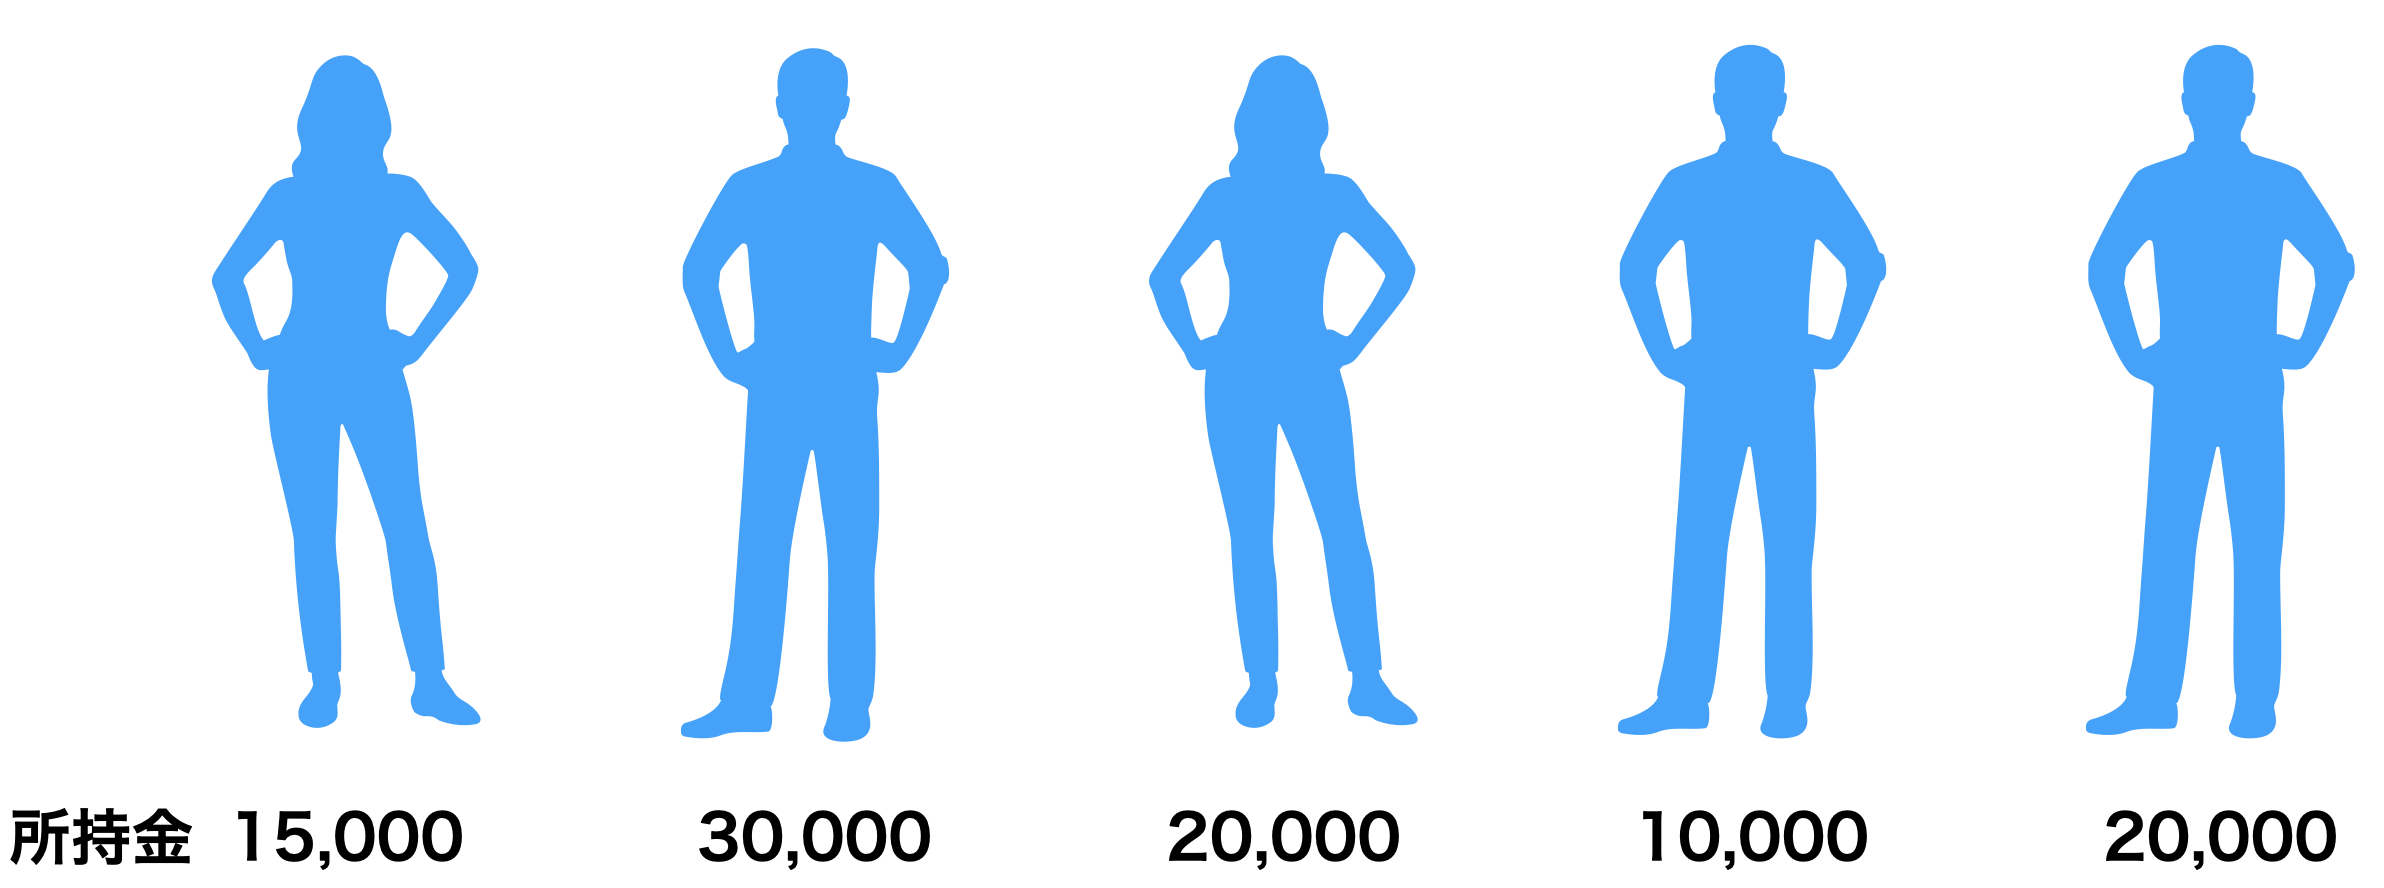
\includegraphics[keepaspectratio,width=0.8\linewidth]{figures/05_descriptives/money.png}
	\caption{5人の所持金データ}
	\label{fig:05_01}
\end{figure}

\paragraph{文字と記号の導入}
さてこれを，今後のために記号で一般的に表記する方法について知っておきましょう。
変数は一般に$x$や$y$で表されます。
今回は5人分のデータがありますが，1人目のデータ，2人目のデータ，といった違いを表すときは$x_1,x_2,\cdots$のようにアルファベットの右斜め下に小さく数字を添えます。添字と言います。
さて今回は所持金という1つの変数でしたが，2つ目の変数，3つ目の変数・・・とたくさんのデータが手に入ることもあります。そのようなとき，変数は$x_{ij}$と添字を2つ書いて表現します。ここで$i$がケース(個体，観測番号)を表し，$j$が何番目の変数であるかを表す，というルールにします\footnote{この講義ではこのルールで通します。必ずしも個体が前で変数が後，という決まりがあるわけではありませんが，このような記号を導入するときはどの文字が何に対応しているか明記することが一般的です。この講義でとくに明記していなければ，前の添字が個体で後ろの添字が変数を表すのだと思ってください。}。

次に足し算の記号を紹介します。$\sum$で総和を表すことにします。この記号はギリシア文字の大文字のSで，足し合わせるsummationの頭文字をとって$\sum$，サムと読みます。この記号には上と下に文字を追加して，次のような意味で使います。
\[ \sum_{i=1}^5 x_i= x_1 + x_2 + x_3 + x_4 + x_5  \]
ここにあるように，$\sum$の下に$i$という文字があります。この文字$i$が$1$から始まって$5$まで変化し総和する，という数学記号です。$\sum_{i=1}^5 x_i$の$x_i$という変数について，$i$が1から5まで変わるわけですから，右辺にあるように添字が変わりながらすべて足し合わせる，という意味の記号です。この$\sum$も，文脈から考えてどこからどこまで足すのかが明らかな場合，上下の添字は省略されることがあります。

さて，先ほどの5人の平均ですが，足し算の場所は$x_1+x_2+\cdots+x_5=\sum_{i=1}^5 x_i$と書けます。これを5で割れば平均になりますから，$\frac{1}{5}\sum x_i = 19000$というわけです。このように記号で表現しておくと，平均値は一般に次のように表すことができます。

\[ \bar{x} = \frac{1}{N}\sum_{i=1}^N x_i \]

今回は5人でしたが，一般に$N$個のデータを扱うときにまで拡張できました。左辺は平均値$\bar{x}$で，エックスバーで表すことが一般的です。
\subsection{中央値median}
次の代表値は\keyterm{中央値}{ちゅうおうち}{median}です。データを大きさの順に並べて行って，ちょうど真ん中のケースの値をその代表値として使う，というものです。さきほどの図\ref{fig:05_01}の場合は，並べ替えると$10000<15000<20000=20000<30000$となります。上から3番目(下からでもいいです)が20000円ですから，中央値は20000円ということになります。

今回はたまたま，5人のケースですから真ん中は3番目となりましたが，データの数が偶数しかなかったらどうするか，という問題があります。その場合は，真ん中に来た2つの値の算術平均でもって中央値とすることが一般的です。

\subsection{最頻値mode}
最後に\keyterm{最頻値}{さいひんち}{mode}についてです。漢字の成り立ちからわかるように，頻度が最も多いものを代表値とするのが最頻値です。さきほどの図\ref{fig:05_01}の場合は，10000円が1人，15000円が1人，30000円が1人ですが20000円持っている人が2人いましたので，最頻値は20000円になります。

このように，データの中心をどのように考えるかによっても3つも考え方があり，それぞれが一致するわけではないのです。それぞれの意義がありますので，見比べながら考える必要があります。

では練習です。次の表\ref{tbl:05_01}のようなデータがあった場合，平均値，中央値，最頻値はそれぞれどうなるでしょう？

\begin{table}[ht]
	\centering
	\caption{5人の所持金データその2}
	\begin{tabular}{lllll}
		A     & B     & C     & D     & E      \\\hline
		10000 & 10000 & 20000 & 25000 & 100000 \\
	\end{tabular}
	\label{tbl:05_01}
\end{table}

この場合，平均は33000円，中央値は20000円，最頻値は10000円となりました。平均値が他の2つより大きくなりましたね。これは\keyterm{外れ値}{はずれち}{outlier}があるからです。Eさんが，平均値をぐっと押し上げているのです。平均値は量的な中心をとりますので，1人でも遠く離れたところに位置すると全体的に中心が引っ張られます。中央値は順番の情報しか使いませんので，大金持ちが1人いても1位だ，と判断するだけです。最頻値は度数の問題ですので，大金持ちが1人いても度数1にしかなりません。平均値は外れ値に弱い，あるいは中央値や最頻値がそれに強いというだけです。

では平均値は使い物にならないのでしょうか？ もちろんそうではなくて，左右対称に散らばっているようなデータであれば，平均値は良い代表値になります。データの分布が左右対称ではなく歪んでいるようであれば，平均値は適切な代表値になりません。

図\ref{fig:05_02}は，厚生労働省による「2023年・国民生活基礎調査」で示されたデータです\footnote{\url{https://www.mhlw.go.jp/toukei/saikin/hw/k-tyosa/k-tyosa23/dl/03.pdf}}。これを見ると所得分布は左側に歪んでおり，平均値は524万2千円ですが，中央値は405万円，最頻値は100-200万円のクラスということになります。最頻値は一番データ点が多いところですので，「国民の平均所得は524万円です」と言われると多くの人が(この例では少なくとも59.6\%の人が)，「えっ，私の年収低すぎ・・・?」という印象を抱きます。もちろん所得分布が低い方に歪んでいる状況も悪いのですが，代表値として平均値を使うことがそもそも適切でない例ともいえます\footnote{もちろん為政者の目から見れば，平均は524万円もあるんだから日本は豊かだ，とアピールできるので良い指標なのかもしれません。数字に悪意はなく，何の数字をどのように使うのかという人の側に問題があるだけです。ちなみにこの数字は2年前の2020年当時から比べて，平均値・中央値ともに下がっています。日本は衰退しました。}。ニュース報道などでは平均値しか報道されませんが，それでは不当な印象を与えることになります。\textbf{データは図にする}ことが大事なのです。
\begin{figure}[ht]
	\centering
	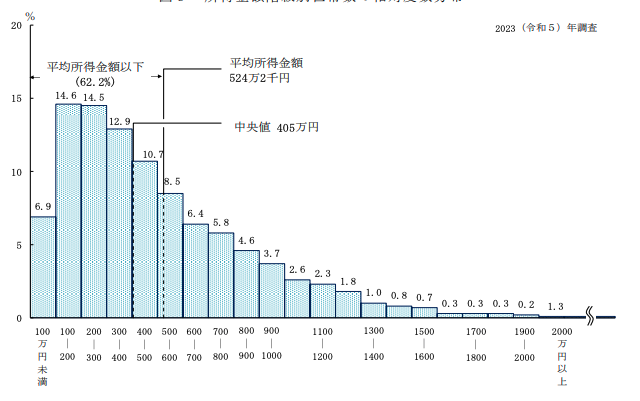
\includegraphics[keepaspectratio,width=0.8\linewidth]{figures/05_descriptives/japanese_2023.png}
	\caption{所得金額階級別世帯数の相対度数分布}
	\label{fig:05_02}
\end{figure}

ところで，最頻値は頻度を数えるものですから，間隔尺度水準以上の連続的な数字の場合はいくつかの区間に区切って数えることになります。図\ref{fig:05_02}の例もそうですね。ただしこの時，最頻値は区間幅の区切り方が違うと結果が変わってしまうことに注意しましょう。図\ref{fig:05_03}の2つのヒストグラムは，実は同じデータなのです。違いは区間幅binwidthのとり方で，左図は15点間隔，右図は5点間隔でグラフを書きました。最頻値はそれぞれ赤で囲ったところになりますが，左図の場合の最頻値は40-55点クラス，右図の場合は47-52点のクラスになります。最頻値の場合は，どのような区間幅でカウントするかということにも注意が必要ですね。
\begin{figure}[ht]
	\centering
	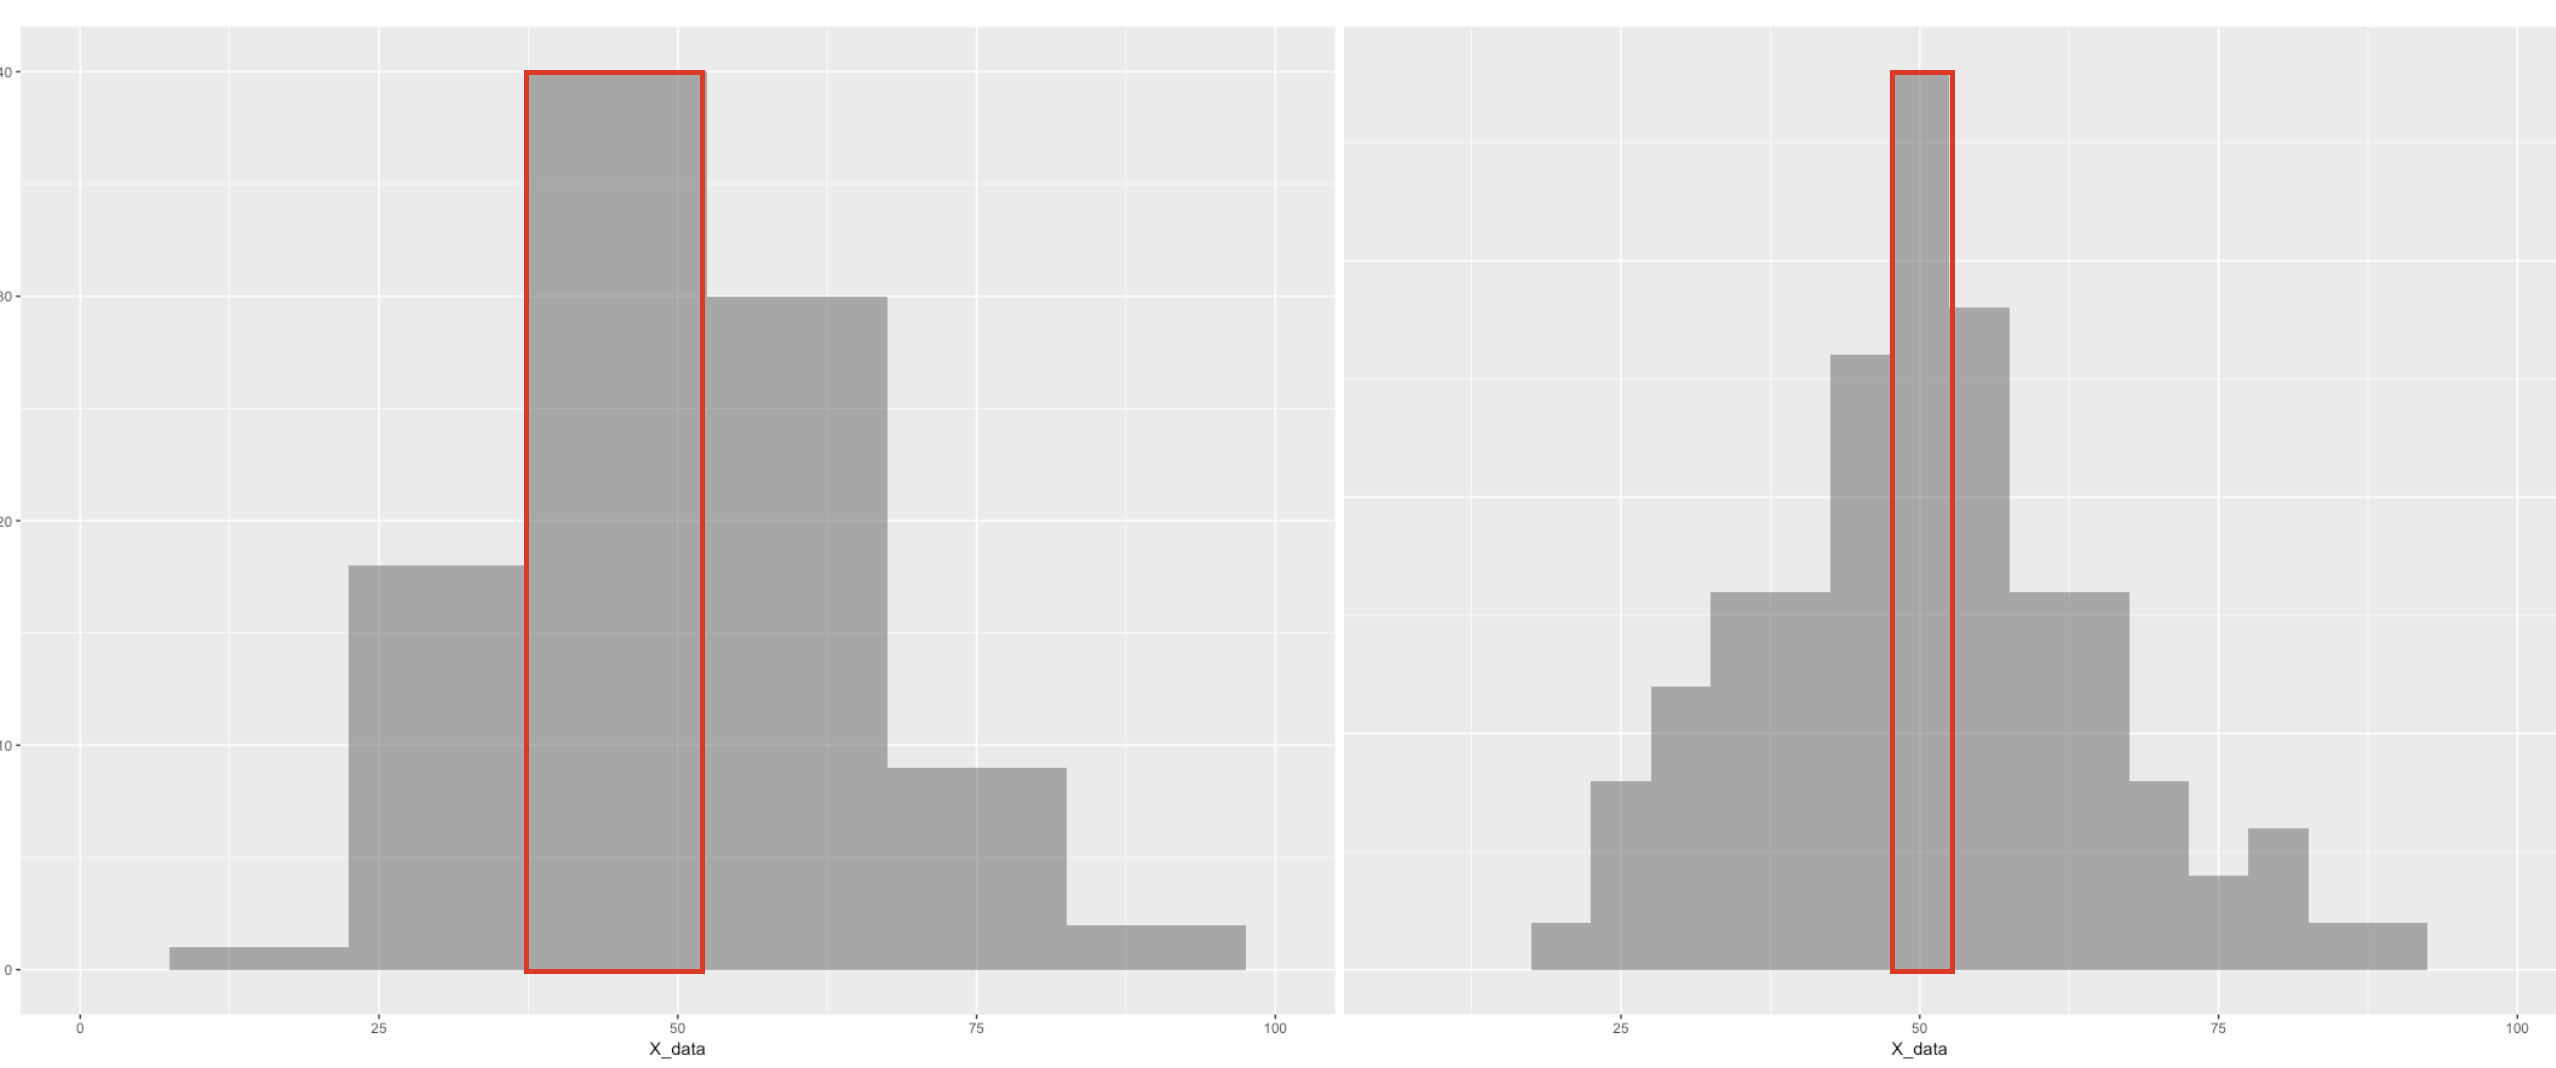
\includegraphics[keepaspectratio,width=0.8\linewidth]{figures/05_descriptives/binwidth.png}
	\caption{区間幅の区切り方で結果が変わる}
	\label{fig:05_03}
\end{figure}

では，ここで出てきた3つの中心化傾向の指標をいったんまとめておきましょう。

\begin{description}
	\item[平均値] データを全部使って計算しており，外れ値がなければ全データが反映される良い指標。実際，統計分析で最も活躍している指標です。左右対称の分布に適しています。
	\item[中央値] 外れ値の影響を受けにくい指標で，ちょうど真ん中，という意味も分かり易いです。ただ，分布の真ん中の数字だけしか使ってません。データが偶数個のときの中央値の計算はいくつかあり得ます。
	\item[最頻値] 外れ値の影響を受けにくく，左右対称でない分布の時も意味が分かり易いです。データの値ではなく度数分布にのみ注目しており，度数分布の区間幅が変わると変わってしまうという欠点があります。
\end{description}

\section{散らばりの指標}
\subsection{分散と標準偏差}
つぎは散らばりの指標について考えていきましょう。データの中心がどこにあるか，というだけではわからないこともあるのです。表\ref{tbl:05_02}のような2つのデータがあったとしましょう。これを図示したのが図\ref{fig:05_04}です。

\begin{table}[ht]
	\centering
	\caption{2つのデータ}
	\begin{tabular}{ll}
		A & B \\\hline
		4 & 1 \\
		4 & 2 \\
		5 & 3 \\
		5 & 5 \\
		5 & 5 \\
		5 & 7 \\
		6 & 8 \\
		6 & 9 \\\hline
	\end{tabular}
	\label{tbl:05_02}
\end{table}

\begin{figure}[ht]
	\centering
	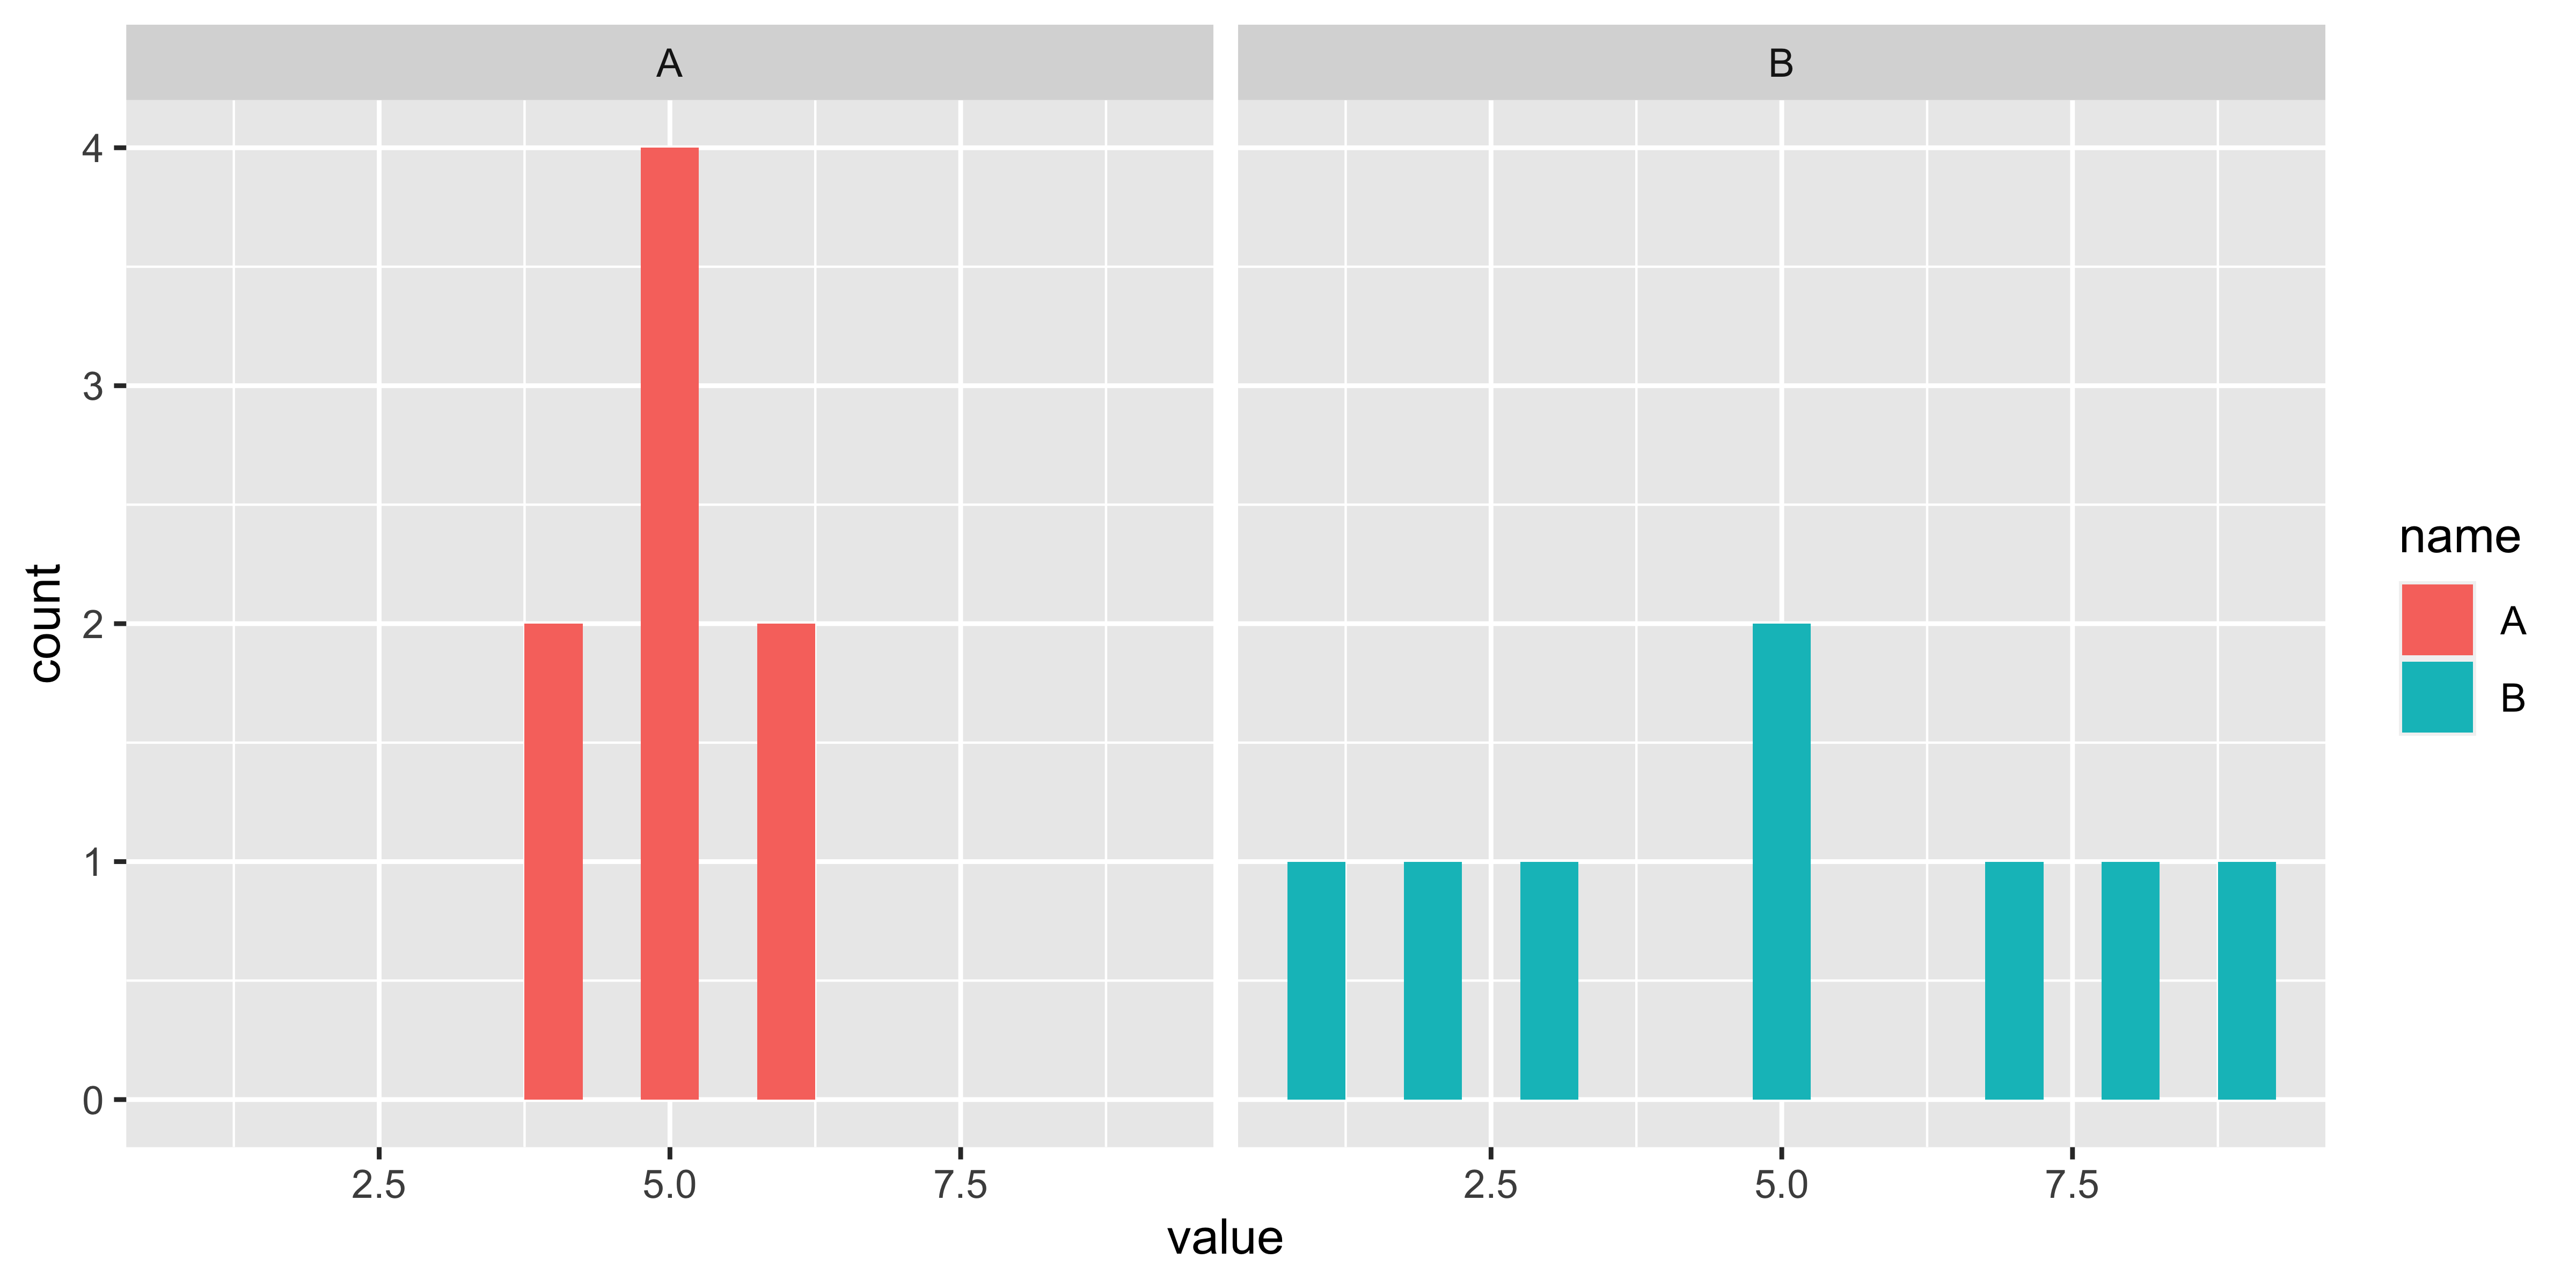
\includegraphics[keepaspectratio,width=0.8\linewidth]{figures/05_descriptives/variance1.png}
	\caption{2つのデータを見比べてみよう}
	\label{fig:05_04}
\end{figure}

このデータ，A/Bグループについてそれぞれ平均値，中央値，最頻値はどうなるでしょう。何と，平均値はA群もB群も5，中央値もA/B群ともに5，最頻値もA/B群ともに5となります。中心化傾向の指標だけでは，A群とB群の違いが表現できません。こんなにも違う見た目をしているのに！

この2つの群は何が違うかといって，図\ref{fig:05_05}を見れば明らかなように中心から左右にどれほど散らばっているかが違うのです。

\begin{figure}[ht]
	\centering
	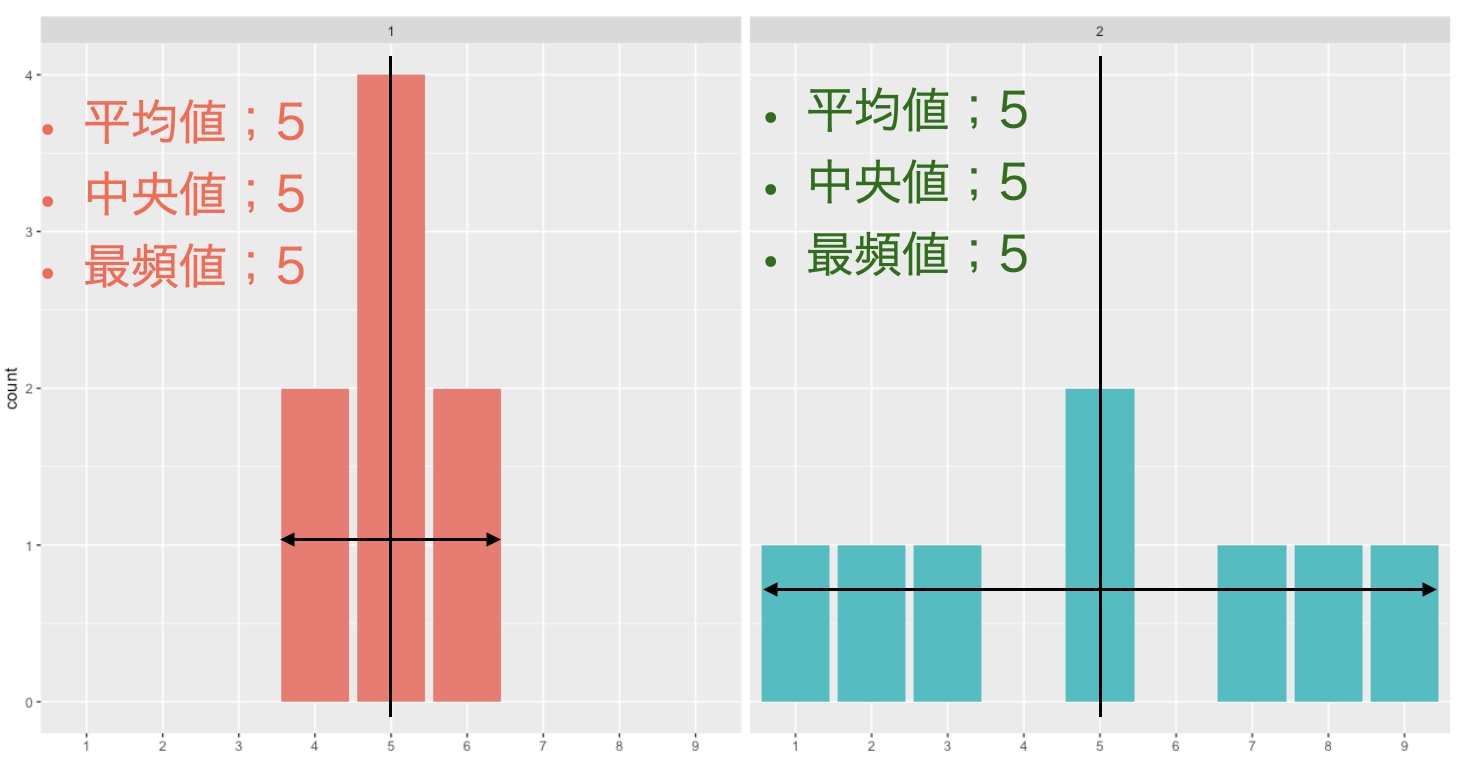
\includegraphics[keepaspectratio,width=0.8\linewidth]{figures/05_descriptives/variance2.png}
	\caption{中心から各データ点が平均的にどの程度離れているか}
	\label{fig:05_05}
\end{figure}

\paragraph{分散}
これをうまく表現する代表値は，\keyterm{分散}{ぶんさん}{variance}があります。指標化のポイントは，「中心から個々のデータ点が平均的にどの程度離れているか」を考慮することにあります。数式では次のように表されます。

\[ s_x^2  = \frac{1}{N}\sum_{i=1}^N (x_i - \bar{x})^2 \]

この式にある$(x_i - \bar{x})$は，各データ点$x_i$が平均$\bar{x}$から離れている程度を表しています。これをとくに\keyterm{平均偏差}{へいきんへんさ}{mean deviation}と言います。それを二乗していますね。これがポイントで，二乗しておかないと平均偏差の総和はゼロになってしまうからです\footnote{検算してみよう!}。プラスとマイナスが打ち消し合うからゼロになってしまうわけで，符号の影響をなくすべく二乗しているのだと思ってください。符号をなくすのには絶対値でもいいのですが，絶対値は数式で書けないから使いにくいのです\footnote{絶対値は$|x|$と書くじゃないか，と思った人もいるかもしれません。おしい，もう一歩。この記号の中身，計算式を考えてみてください。$0\le x$のとき，$|x|=x$です。$x<0$のとき，$|x|=-x$です。これ，「・・・の時」という条件で分岐してて，この箇所が数式で書けてないですよね。}

実際に計算してみましょうか。A群の分散は，次のようになります。
\[ \frac{1}{8}((4-5)^2+(4-5)^2+(5-5)^2+(5-5)^2+(5-5)^2+(5-5)^2+(6-5)^2+(6-5)^2) \]
\[ =\frac{1}{8}(1^2+1^2+0^2+0^2+0^2+0^2+1^2+1^2) = \frac{4}{8}=0.5\]
B群の分散は，次のようになります。
\[ \frac{1}{8}((1-5)^2+(2-5)^2+(3-5)^2+(5-5)^2+(5-5)^2+(7-5)^2+(8-5)^2+(9-5)^2)\]
\[ =\frac{1}{8}(4^2+3^2+2^2+0^2+0^2+2^2+3^2+4^2) = \frac{58}{8}=7.25 \]
このように，A群の分散は0.5，B群の分散は7.25と，B群の方が散らばりが大きいことがわかります。

分散はデータの散らばりを表現しています。分散が大きい方がデータの散らばりが大きい，というわけですね。
逆に分散がゼロになると，そのデータには散らばりがない，ということです。
実際取ったデータの分散がゼロだと，そこから得られる情報がない，ということになります。
なぜなら，たとえばクラスの全員がテストで100点を取ると，分散は0です。この時は「どういう勉強をすれば成績が上がるか」とか「成績が低い人をどうサポートすれば良いか」という知見を得ることができません。分散が0のデータセットには，個々の違いがないので情報が得られないのです。つまり，分散はそのデータから取り出せる「意味」「情報」の上限という点で非常に重要な指標なのです！

ちなみに分散の式は，次のように展開できます。
\[
	\begin{array}{lllr}\label{ref:variance_form2}
		s_x^2 & = & \frac{1}{N}\sum_{i=1}^N (x_i - \bar{x})^2                                                                                           \\
		\\
		      & = & \frac{1}{N}\sum_{i=1}^N (x_i^2 - 2x_i\bar{x} + \bar{x}^2)                                                                           \\
		      &   &                                                                                                          & \mbox{$\sum$ 記号は分配できるから} \\
		      & = & \frac{1}{N}\sum_{i=1}^N x_i^2 - 2\frac{1}{N}\sum_{i=1}^N x_i\bar{x} + \frac{1}{N}\sum_{i=1}^N \bar{x}^2)                            \\
		      &   &                                                                                                          & \mbox{定数をN回足すのはN倍と同じなので} \\
		      & = & \frac{1}{N}\sum_{i=1}^N x_i^2 - 2\frac{1}{N}N\bar{x}\sum_{i=1}^N x_i + \frac{1}{N}N\bar{x}^2)                                       \\
		      &   &                                                                                                                                     \\
		      & = & \frac{1}{N}\sum_{i=1}^N x_i^2 - 2\bar{x}\frac{1}{N}\sum_{i=1}^N x_i + \bar{x}^2)                                                    \\
		      &   &                                                                                                                                     \\
		      & = & \frac{1}{N}\sum_{i=1}^N x_i^2 - 2\bar{x}\bar{x}+ \bar{x}^2)                                                                         \\
		      &   &                                                                                                                                     \\
		      & = & \frac{1}{N}\sum_{i=1}^N x_i^2 - 2\bar{x}^2+ \bar{x}^2)                                                                              \\
		      &   &                                                                                                                                     \\
		      & = & \frac{1}{N}\sum_{i=1}^N x_i^2 - \bar{x}^2
	\end{array}
\]
て計算するときなどは，先に全ての変数を二乗したり，変数の平均の計算をしたりしますので，こちらの方が計算が早くなるかもしれません。もっとも電子計算機の発展している現代において，手計算で分散を求めることなんか少なくなりましたけどね。
\paragraph{標準偏差}
ところで，分散は元のデータを二乗した値から計算しているのでした。ですから，その単位が元の尺度と異なることに注意が必要です。つまり，元がcm位のデータであれば，分散は$cm^2$の単位になっているのです。ですから数字が必然的に大きくなりがちですし，分散の大きさが実際どれぐらいなのか，という実感が持ちにくいという欠点があります。

そこで，単位を元に戻すことを考えます。二乗して大きくなっているのですから，平方根をとってやれば元に戻りますね。
\[ s_x = \sqrt{\frac{1}{N}\sum_{i=1}^N (x_i - \bar{x})^2} \]
このようにして計算された$s_x$のことを\keyterm{標準偏差}{ひょうじゅんへんさ}{standard deviation}(SD)と言います。これはルートを取るだけですので，すぐに計算できますね。さきほどの例ですと，A群のSDは0.7071，B群のSDは2.6925です。


\paragraph{\ruby{四分位}{しぶんい}数 とIQR}
他にも範囲を表現する指標はあります。分散や標準偏差が平均値に関する指標であったのに対し，中央値に関係した指標として\keyterm{四分位}{しぶんい}{Quantile}というのがあります。文字通り，データを四分割した時の切れ目にあたる数字のことです。
中央値はデータを大きい順に並べ替えて，ちょうど真ん中になる数字という話でしたが，四分割した場合は図\ref{fig:05_06}にあるように，下の方が第1四分位，上の方が第3四分位ということになります。中央値は第2四分位と同じことになるのですね。

\begin{figure}[ht]
	\centering
	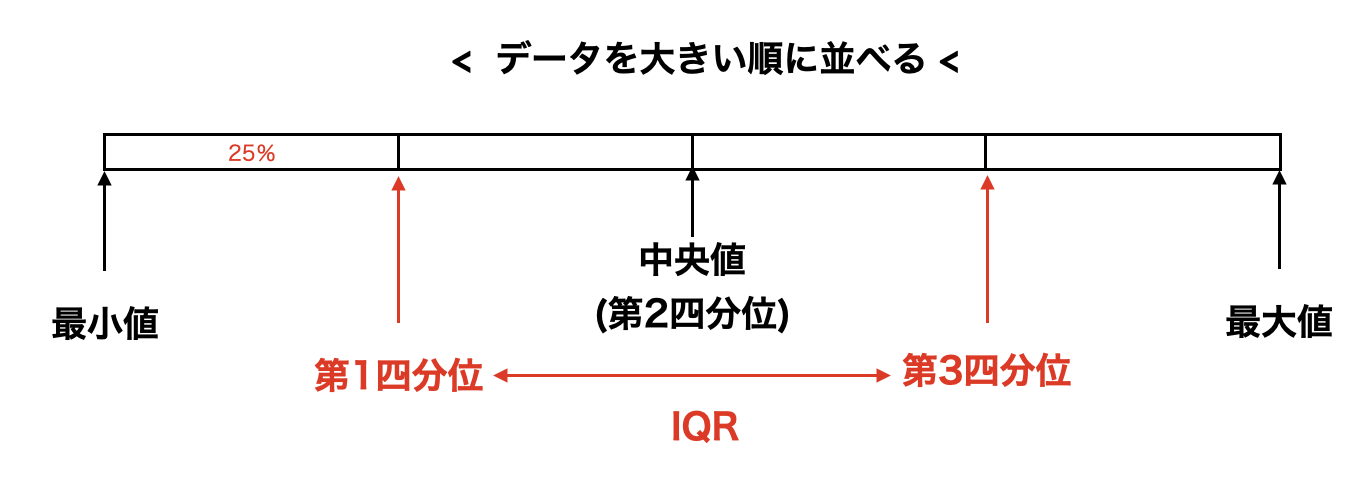
\includegraphics[keepaspectratio,width=0.8\linewidth]{figures/05_descriptives/iqr.png}
	\caption{四分位とIQR}
	\label{fig:05_06}
\end{figure}

この第1と第3をつかった幅，つまり第3四分位数から第1四分位数を引いた数字のことを\keyterm{四分位範囲}{しぶんいはんい}{Inter-Quartile Range IQR}と呼びます。中央値と同じように外れ値の影響を受けにくく，また標準偏差のように元データと同じ単位ですので，理解しやすい指標です。
さてここで，四分割じゃなくて五分割がいい，と思った人もいるかもしれません。いや三分割でも何分割でもいいんですが，要するになんらかの割合で区切った値というのを考えることは可能ですよね。この「割合に応じた値」のことを，\keyterm{パーセンタイル}{ぱーせんたいる}{Percentile}と言います。たとえば第1四分位は25パーセンタイル，第3四分位は75パーセンタイルと同じ意味です。この表現が使えるのなら，任意の数字で分割できるのでいいですね。分布の形状によっては，95パーセンタイルとか5パーセンタイルといった値を表示することもあります\footnote{テスト理論業界では，\keyterm{スタナイン}{すたないん}{Stanine}という区切り型もあります。全体を均等に9区分するのではなく，上から順に4\%,7\%,12\%,17\%,20\%,17\%,12\%,7\%,4\% で区切ります。一桁で表現できる均等な区切りであり，この不均一な数字は学力の分布が正規分布に従うことから来ています。詳しくは，\textcite{TDE2022}を参照してください。}。

\paragraph{最大値，最小値，範囲}
次に最も簡単な散らばりを示す数値を紹介します。\keyterm{最大値}{さいだいち}{Max}はデータのなかで一番大きな値を指します。\keyterm{最小値}{さいしょうち}{Min}は逆に，データの中で一番小さな値です。\keyterm{範囲}{はんい}{Range}は最大値から最小値を引いたものです。これは単純ですね。


さてここまでで，中心化傾向の指標と散らばりの指標について説明してきました。冒頭でお伝えしたように，これらの代表値は1つだけで表現できることに限界があります。論文などでは，取得したデータについての記述統計量をまず記載することが基本です。データの平均値，中央値，標準偏差，最大値と最小値などを記載することで，どういうデータだったかが(データ点すべてを書かなくても)見えてきます。逆にいうと，平均値だけではデータの真ん中を示すだけですし，歪んだデータになっているかもしれないことが読み取れません。ちなみにデータが左右対称でない場合，よく使われる統計的分析手法が適用できないこともあります。それを無視してデータを分析すると，間違った結論に辿り着くかもしれないのです。データをさまざまな角度でみる(描画し，複数の代表値を確認する)ことを厭わないでください。幸い，多くの統計パッケージはすぐにこれらの指標を算出してくれますので，計算の苦労はありません。

\section{Rによる集計}

では具体的にRをつかって計算をしてみましょう。

まずは計算に先立って，この授業のプロジェクトを開き，新しいスクリプトファイルを用意してください。
また，プロジェクトフォルダにサンプルデータをダウンロードし，同プロジェクトフォルダに保存してください。
サンプルデータはこの講義の伴走サイト\footnote{\url{https://kosugitti.github.io/psychometrics_syllabus/}}からダウンロードできます。

新しいスクリプトファイルに次のコードを書いて，データを\verb|dat|に読み込んでください。
\begin{lstlisting}[language=c++,label={code:5_01},caption={データの読み込み}]
rm(list = ls())
library(tidyverse)
dat <- read.csv("BaseballDecade.csv",na.strings = "NA")
dat2011 <- dat %>% filter(Year == "2011年度")
\end{lstlisting}

\paragraph{コード解説}
\begin{description}
	\item[1行目] 環境変数のクリア。Rの頭の中をまず空っぽにします！
	\item[2行目] \verb|tidyverse|パッケージを読み込みます。データ操作や描画に便利な関数がたくさん入っています。
	\item[3行目] \verb|read.csv|関数で，カンマ区切りのCSVファイルを読み込みます。欠損値は\verb|NA|として読み込みます。
	\item[4行目] \verb|tidyverse|パッケージに含まれる\verb|filter|関数\footnote{正確には，\verb|tidyverse|パッケージは便利なパッケージのパッケージで，\verb|filter|関数は\verb|tidyverse|パッケージが読み込む\verb|dplyr|パッケージのもつ関数です。}で，2011年度のデータだけを抽出して\verb|dat2011|に格納します。
\end{description}


実践的にはこのように，外部ファイルからデータを読み込むことが一般的です。
すでにみたように，データの構造を確認するためには\verb|str()|関数を使えばよいのですが，データの中身を確認するためには，データの中身を確認するためには\verb|head()|関数を使えばよいです。

\begin{lstlisting}[language=c++,label={code:5_02},caption={データの確認}]
str(dat2011)
head(dat2011)
\end{lstlisting}

\begin{Rscreen}{データの確認}{check}
\begin{verbatim}
> str(dat2011)
'data.frame':	626 obs. of  17 variables:
 $ Year      : chr  "2011年度" "2011年度" "2011年度" "2011年度" ...
 $ Name      : chr  "永川　勝浩" "前田　健太" "栗原　健太" "東出　輝裕" ...
 $ team      : chr  "Carp" "Carp" "Carp" "Carp" ...
 $ salary    : int  12000 12000 12000 10000 9000 8000 8000 7500 7000 6600 ...
 $ bloodType : chr  "O型" "A型" "O型" "A型" ...
 $ height    : int  188 182 183 171 201 183 177 173 176 188 ...
 $ weight    : int  97 73 95 73 100 90 82 73 80 97 ...
 $ UniformNum: int  20 18 5 2 70 17 31 6 1 43 ...
 $ position  : chr  "投手" "投手" "内野手" "内野手" ...
 $ Games     : int  19 31 144 137 19 6 110 52 52 40 ...
 $ AtBats    : int  NA NA 536 543 NA NA 299 192 44 149 ...
 $ Hit       : int  NA NA 157 151 NA NA 60 41 11 35 ...
 $ HR        : int  NA NA 17 0 NA NA 4 2 0 1 ...
 $ Win       : int  1 10 NA NA 0 1 NA NA NA NA ...
 $ Lose      : int  2 12 NA NA 0 1 NA NA NA NA ...
 $ Save      : int  0 0 NA NA 0 0 NA NA NA NA ...
 $ Hold      : int  0 0 NA NA 9 0 NA NA NA NA ...
> head(dat2011)
      Year       Name team salary bloodType height weight UniformNum
      position Games AtBats Hit HR Win Lose
1 2011年度 永川　勝浩 Carp  12000       O型    188     97         20     投手    19     NA  NA NA   1    2
2 2011年度 前田　健太 Carp  12000       A型    182     73         18     投手    31     NA  NA NA  10   12
3 2011年度 栗原　健太 Carp  12000       O型    183     95          5   内野手   144    536 157 17  NA   NA
4 2011年度 東出　輝裕 Carp  10000       A型    171     73          2   内野手   137    543 151  0  NA   NA
5 2011年度   シュルツ Carp   9000      不明    201    100         70     投手    19     NA  NA NA   0    0
6 2011年度   大竹　寛 Carp   8000       B型    183     90         17     投手     6     NA  NA NA   1    1
  Save Hold
1    0    0
2    0    0
3   NA   NA
4   NA   NA
5    0    9
6    0    0
\end{verbatim}
\end{Rscreen}

さて，このようにデータが読み込めたら，そのデータの特徴をみるために，記述統計量を算出してみましょう。まずはデータ全体の傾向を見るための，\verb|summary()|関数を使ってみましょう。

\begin{lstlisting}[language=c++,label={code:5_03},caption={記述統計量の算出}]
summary(dat2011)
\end{lstlisting}

量的な変数に対して，最小値(\verb|Min|)，第1四分位数(\verb|1st Qu.|)，中央値(\verb|Median|)，平均値(\verb|Mean|)，第3四分位数(\verb|3rd Qu.|)，最大値(\verb|Max|)が表示されていると思います。
\verb|factor|型にしておいた変数があれば，その度数を表示してくれているはずです。

\section{Rによる統計量の算出}
これでも大体の概略はわかるのですが，もう少し詳しくデータの特徴をみてみましょう。この講義で学んだ記述統計量をひとつひとつ算出して行きます。

以下では例として，\verb|salary|変数の記述統計量を算出してみます。オブジェクトの特定の変数を参照するには，\verb|$|を使うことを思い出してください。

まずは平均値です。平均値は\verb|mean()|関数で算出できます。

\begin{lstlisting}[language=c++,label={code:5_04},caption={平均値の算出}]
mean(dat2011$salary)
\end{lstlisting}

欠損値があるデータの場合は，オプションとして\verb|na.rm = TRUE|を指定します。ホームランの本数の平均値を算出してみましょう。

\begin{lstlisting}[language=c++,label={code:5_04_2},caption={平均値の算出}]
mean(dat2011$HR, na.rm = TRUE)
\end{lstlisting}


中央値は\verb|median()|関数で算出できます。

\begin{lstlisting}[language=c++,label={code:5_05},caption={中央値の算出}]
median(dat2011$salary)
\end{lstlisting}

分散は\verb|var()|関数で，標準偏差は\verb|sd()|関数で算出できます。ただし，これらの関数は上で定義した分散，標準偏差を算出するものではないことに注意してください。詳しくは後の方で説明することになりますが，分散の式の中であった$\frac{1}{N}$の部分が，これらの関数では$\frac{1}{N-1}$になっているのです\footnote{どうしてそうなるのかについては，推測統計学の講義で説明します。$N-1$で割る分散のことを不偏分散，$N$で割る分散のことを標本分散といい，デフォルトの関数では不偏分散の方を算出するということを頭の片隅に置いておくようにしてください。}。

\begin{lstlisting}[language=c++,label={code:5_06},caption={分散と標準偏差の算出}]
var(dat2011$salary)
sd(dat2011$salary)
\end{lstlisting}

最大値は\verb|max()|関数で，最小値は\verb|min()|関数で算出できます。

\begin{lstlisting}[language=c++,label={code:5_07},caption={最大値と最小値の算出}]
max(dat2011$salary)
min(dat2011$salary)
\end{lstlisting}

最後に，四分位数を算出してみましょう。

\begin{lstlisting}[language=c++,label={code:5_08},caption={四分位数の算出}]
quantile(dat2011$salary)
\end{lstlisting}

\begin{Rscreen}{四分位数の算出}{quantile_R}
\begin{verbatim}
> quantile(dat2011$salary)
   0%   25%   50%   75%  100% 
  400  1000  2000  5500 50000 
\end{verbatim}
\end{Rscreen}

このように，四分位数は0\%,25\%,50\%,75\%,100\%の5つの値で表されています。50\%の値は中央値と同じことを確認してください。なお，\verb|quantile()|関数は，デフォルトでは四分位数を算出しますが，引数を指定することで，任意のパーセンタイルを算出することも可能です。すなわち，30\%のパーセンタイル点，75\%のパーセンタイル点などを算出することも可能です。

\begin{lstlisting}[language=c++,label={code:5_09},caption={任意のパーセンタイルの算出}]
quantile(dat2011$salary, probs = c(0.3, 0.75))
\end{lstlisting}

\begin{Rscreen}{任意のパーセンタイルの算出}{percentile_R}
\begin{verbatim}
> quantile(dat2011$salary, probs = c(0.3, 0.75))
 30%  75% 
1200 5500 
\end{verbatim}
\end{Rscreen}

\section{Rによるデータの可視化}

これらの関数を応用することで，データの各変数について様々な記述統計量を確認することができるようになりました。しかし，\textbf{データは図にする}ことで，より理解しやすくなります。というか，データを図にしなければ，データの特徴をみることはできません。

まずは，データの分布を視覚的に理解するために，ヒストグラムを描画してみましょう。ヒストグラムは\verb|hist()|関数で描画できます。

\begin{lstlisting}[language=c++,label={code:5_10},caption={ヒストグラムの描画}]
hist(dat2011$salary)
\end{lstlisting}

出力された図を見ると，非常に偏った分布になっていることがわかります。これに対して，身長や体重のデータは比較的左右対称の形になっていることがわかります。  

\begin{figure}[ht]
	\centering
	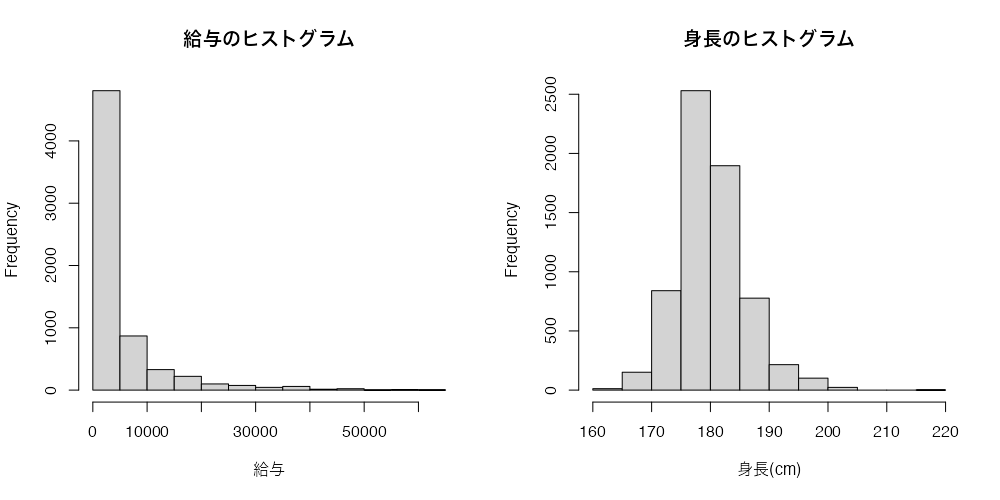
\includegraphics[keepaspectratio,width=0.8\linewidth]{figures/05_descriptives/hist_func.png}
	\caption{ヒストグラムの描画}
\end{figure}

このように，ヒストグラムは単一の変数の分布を視覚的に確認する時に有用です。

次に，\keyterm{箱ひげ図}{はこひげず}{boxplot}を描画してみましょう。箱ひげ図は\verb|boxplot()|関数で描画できます。

\begin{lstlisting}[language=c++,label={code:5_11},caption={箱ひげ図の描画}]
boxplot(dat2011$salary)
\end{lstlisting}

この箱ヒゲ図，別名ボックスプロットも，変数の分布を確認する表示の仕方です。もしかすると皆さんはすでに，高校までの数学で学んだことがあるかもしれません。この図示の方法は，データがどのぐらいの幅を持っているかを箱とひげで表現しています。箱の真ん中にあるのが中央値，箱の下のラインが第1四分位，上のラインが第3四分位を表すのが一般的です。ですが，髭に当たる部分については2通りの書き方があります。図\ref{fig:05_07}にあるのは同じデータですが，ひげの長さを「最大値から最小値まで」とする方法(上段)もありますし，「IQRの1.5倍まで」とする方法(下段)もあります。どちらの方法で描画されているのか，注意するようにしてください\footnote{高校数学，引いてはセンター試験などでは最大値から最小値まで表す，という記法が使われているようですが，データ分析の文脈ではIQRの1.5倍までをひげにして，それ以上の数字は外れ値として点で表す方法が一般的です。どちらが正しいとも言えないのですが，今後は後者の書き方に出会うことの方が多いと思いますので，注意を促すために書いています。}。
\begin{figure}[ht]
	\centering
	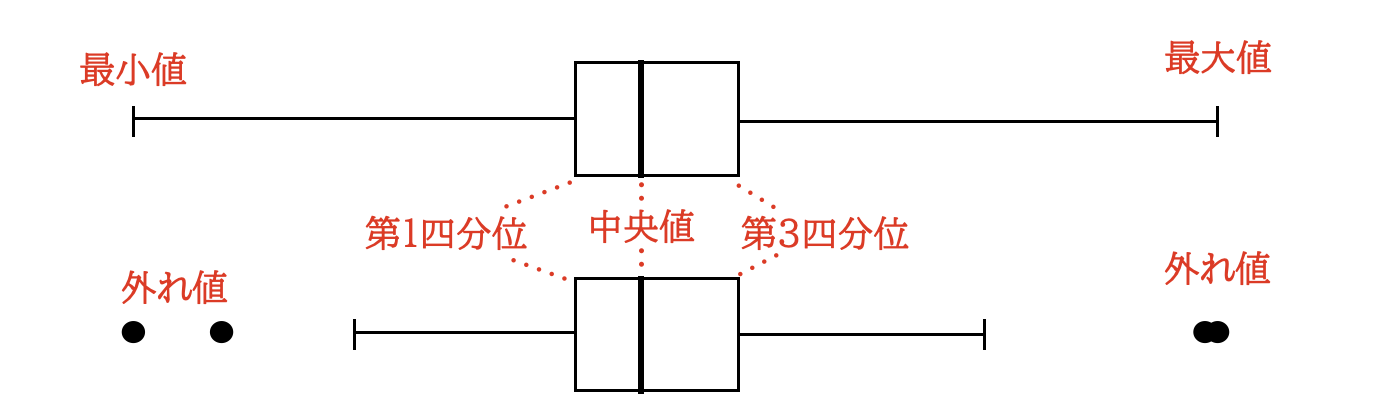
\includegraphics[keepaspectratio,width=0.8\linewidth]{figures/05_descriptives/boxplot.png}
	\caption{ボックスプロット(箱ひげ図)の2通りの書き方}
	\label{fig:05_07}
\end{figure}


\section{課題}
今回の課題は，以下の計算をするRスクリプトファイルを提出してください。
ファイル名は学籍番号と氏名を含むものとし，拡張子は\verb|.R|にしてください。
\textbf{提出するファイルはエラーのない完備な.Rファイルにしてください。}
ファイル形式の間違い，出力にエラーが含まれている(未完成な)ものは返却しますので注意してください。

課題の内容は次のとおりです。
\begin{enumerate}
	\item サンプルデータ\texttt{BaseballDecade.csv}をダウンロードし，プロジェクトフォルダに保存します。
	\item 名義尺度水準のデータの変数を全て\verb|factor|型に変換してください。\verb|Name|変数は名義尺度水準でなくて構いません。
	\item データ全体の要約をする関数\verb|summary|を使って，データオブジェクトの記述統計量を表示してください。
	\item 年俸\verb|salary|と安打数\verb|Hit|の平均値，中央値，最大値，最小値，IQR，5パーセンタイル点，95パーセンタイル点を算出してください。
	\item 年俸の箱ヒゲ図を描いてください。
\end{enumerate}


\newpage
\section{補遺}
本章で出てきた，\verb|tidyverse|パッケージについて，すこし説明を追加しておきましょう。

\subsection{データハンドリング}
\label{dataHandling}

データハンドリングとは，データを加工するという意味です。進んだ統計的な分析などをする場合も，まずは元のデータを分析しやすい形に整える作業が必要なのです。

面白いもので，このデータハンドリングだけについて書かれた本もあります。\textcite{Kinosady2021}がそうで，どんなデータをどのように分析するか，について触れることなく，どのようにデータを加工するか，加工しやすくするための準備をするか，ということに特化しています。手元に一冊置いておきたいおすすめの一冊です。

ここではよく使われる基本的な関数を抜粋して，ご紹介します。

\paragraph{tidyverseパッケージ}
ここでは\verb|tidyverse|パッケージと呼ばれる，データハンドリング専門パッケージの使い方を説明していきます。このパッケージは，パッケージをひとまとめにしたパッケージです。つまり便利グッズのパッケージ，「初心者お料理セット」みたいなものですね。

インストールは前回(セクション\ref{HowToUseRpackage},Pp.\pageref{HowToUseRpackage})で既に終わっているでしょうから，これを読み込んでハンドリングしてみましょう。
ダウンロードとインストールは同じ環境で1回やれば終わりますので，起動するたび，実行するたびに毎回行う必要はありませんが，実行に際してはパッケージを\textbf{実装}しなければなりません。ダウンロードとインストールはグッズの購入であって，実装とはそのグッズを身につけるということですね\footnote{ドラゴンクエストというゲームでは，武器や防具を武器屋で買いますが，買って持っているだけでは身につけたことになりませんし，当然その効果も発動しません。購入した武器や防具を「身に着ける」というアクションが必要です。武器屋で購入すると，店主が「ここで身につけていくかい」というセリフで注意喚起してくれます。}。
実装する関数は\verb|library|で，実行すると図\ref{RS:library_tidyverse}のように表示されます。

\begin{Rscreen}{tidyverseパッケージの読み込み}{library_tidyverse}
	\begin{verbatim}
> library(tidyverse)
── Attaching core tidyverse packages ────────────────────── tidyverse 2.0.0 ──
[v] dplyr     1.1.4     [v] readr     2.1.5
[v] forcats   1.0.0     [v] stringr   1.5.1
[v] ggplot2   3.5.2     [v] tibble    3.2.1
[v] lubridate 1.9.4     [v] tidyr     1.3.1
[v] purrr     1.0.4     
── Conflicts ─────────── tidyverse_conflicts() ──
[x] dplyr::filter() masks stats::filter()
[x] dplyr::lag()    masks stats::lag()
[i] Use the conflicted package to force all conflicts to become errors
\end{verbatim}
\end{Rscreen}
ここに示されているのは，\verb|dplyr, readr, forcats, stringr, ggplot2, tibble, lubridate, tidyr, purrr|というパッケージを読み込みましたよ，ということと，読み込んだ\verb|dplyr|パッケージの\verb|filter|関数と\verb|lag|関数が他のパッケージと干渉(conflict)しているので，上書きしましたよということです。基本的に気にしなくてよい情報です\footnote{とは言え気になる人のために。パッケージは数多くありますから，あるパッケージAで使う関数と，あるパッケージで使う関数が同じ名前だった，ということがあり得るわけです。これが「名前空間の干渉」というやつで，これを解消するためには，Aパッケージの関数fだよ，Bパッケージの関数fだよ，ということを明示してやる必要があります。Rではコロンを2つ繋げて，\verb|A::f()|とすることでAパッケージの関数fを表しています。ここでは\verb|dplyr::filter()|が\verb|stats::filter()|をマスクしましたよ，ということを意味しており，パッケージの指定なしで\verb|filter()|と書くとこの後は\verb|dplyr()|パッケージの\verb|filter()|を使いますよ，ということです。このあとも\verb|stats|パッケージの\verb|filter()|を使いたい場合は，\verb|stats::filter()|とすればOKです。ちなみに\verb|stats|パッケージとは，Rを起動した段階で読み込まれている基本中の基本パッケージです。}。

ところで，先ほどの\verb|read_csv|関数を実行すると図\ref{RS:readcsv}のような出力が出てくるかと思います。
赤い文字なのでエラーだ！と思って驚くかもしれませんが，よくみてください。6546行(Rows)，17列(Columns)とあるように，データのサイズが表示されています。続く表示も，区切り文字がカンマであること(\verb|Delimiter: ","|)，文字列の変数と数値(dbl)の変数\footnote{\verb|dbl|はダブルdouble，つまり倍精度の長さを持つ実数変数だということです。要するに数字です。}であることなどがでています。これはエラーではなくて，正しく読み込めているかどうか確認するためのメッセージなのです。親切！

\begin{Rscreen}{外部データの読み込み時メッセージ}{readcsv}
\begin{verbatim}
> dat <- read_csv("BaseballDecade.csv",na = "NA")
Rows: 6546 Columns: 17                                                                             
── Column specification ──────────────────────
Delimiter: ","
chr  (6): Year, Name, team, bloodType, UniformNum, position
dbl (11): salary, height, weight, Games, AtBats, Hit, HR, Win, Lose, Save, Hold

[i] Use `spec()` to retrieve the full column specification for this data.
[i] Specify the column types or set `show_col_types = FALSE` to quiet this message.
\end{verbatim}
\end{Rscreen}

さあでは\verb|tidyverse|パッケージをつかってデータハンドリングしてみましょう。
今からいくつかの関数を紹介します。それらはレゴブロックの1ピースのようなもので，「これだけ渡されてもどうしろと」と思うかもしれませんが，これらを組み合わせると大きなことができる・・・！と思ってお付き合いください。
\paragraph{列選択：select}
まずは列選択の関数，\verb|select|について。先ほど読み込んだ野球データは出力\ref{RS:check}にあるように多くの変数があります。ここから，身長\verb|height|と体重\verb|weight|だけの変数を取り出したい，というときにこの関数を使います。
コード\ref{code:usingR_select}の結果が出力\ref{RS:usingR_select}です。
\begin{lstlisting}[language=c++,label={code:usingR_select},caption={select関数}]
dat %>% select(height,weight)
\end{lstlisting}
\begin{Rscreen}{select関数の出力結果}{usingR_select}
	\begin{verbatim}
> dat %>% select(height,weight)
# A tibble: 6,546 × 2
   height weight
    <dbl>  <dbl>
 1    188     97
 2    182     73
 3    183     95
 4    171     73
 5    201    100
 6    183     90
 7    177     82
 8    173     73
 9    176     80
10    188     97
# [i] 6,536 more rows
# [i] Use `print(n = ...)` to see more rows
\end{verbatim}
\end{Rscreen}
変数が2つに絞られていることが確認できますね。

ここで重要なポイントがあります。それはパイプ演算子\verb|%>%|です。これは前のオブジェクトを後の関数の第一引数に渡す，という意味があります。たとえば，$y=f(x)$という変換をし，さらに$z=g(y)$という変換をしたい場合，頭の中では$x\to y \to z$と考えていると思いますが，コードで書くと$y \leftarrow x$で$z \leftarrow y$という逆の向きで考えなければなりません。あるいは$z=g(f(x))$と内側にくり入れていくので，見た目にわかりにくくなります。この思考の流れに沿った変換にするようにつなげるのが\verb|%>%|です\footnote{これを読むときは，頭の中で「経て」と読みましょう。\verb|dat|を経て\verb|select|へ。なんのこっちゃと思った人は，ダウンタウンのごっつええ感じという昔の番組で「経て」というコントがあったので，ググってみてみてください。}\footnote{パーセント，大なり，パーセントと3回も入力するのは面倒ですね！RStudioではショートカットキーとして，\verb|Ctrl+Shift+M|があります。CtrlキーとShiftキーとMを同時押し，です。こうした入力ショートカットについては他にもいろいろあり，RStudioのHelpメニューからCheetSheetを選択してください。チートコマンドを書き込んださまざまな情報が1-2枚にまとまっています。}。

\paragraph{行選択：filter}
今度は行選択。\verb|filter|という関数です。先ほど読み込んだデータは6546行もあるのですが，たとえば2020年度のデータだけが欲しい，というときは行を選択することになります。ここで使うのが\verb|filter|です。コード\ref{code:usingR_filter}の結果が出力\ref{RS:usingR_filter}です。
\begin{lstlisting}[language=c++,label={code:usingR_filter},caption={filter関数}]
dat %>% filter(Year == "2020年度")
\end{lstlisting}
\begin{Rscreen}{filter関数の出力結果}{usingR_filter}
	\begin{verbatim}
> dat %>% filter(Year == "2020年度")
# A tibble: 664 × 17
   Year     Name    team  salary bloodType height weight UniformNum
   <chr>    <chr>   <chr>  <dbl> <chr>      <dbl>  <dbl> <chr>     
 1 2020年度 菊池　涼介…… Carp   30000 A型          171     72 33        
 2 2020年度 鈴木　誠也…… Carp   28000 A型          181     98 1         
 3 2020年度 Ｋ．ジョンソ… Carp   27250 不明         193     95 42        
 4 2020年度 會澤　翼…… Carp   18000 B型          177     91 27        
 5 2020年度 大瀬良　大地… Carp   17500 AB型         187     95 14        
 6 2020年度 長野　久義…… Carp   17000 O型          180     85 5         
 7 2020年度 田中　広輔…… Carp   15000 A型          171     84 2         
 8 2020年度 中﨑　翔太…… Carp   14500 B型          186     99 21        
 9 2020年度 野村　祐輔…… Carp   12000 AB型         177     89 19        
10 2020年度 松山　竜平…… Carp    8500 B型          176     96 55        
# [i] 654 more rows
# [i] 9 more variables: position <chr>, Games <dbl>, AtBats <dbl>,
#   Hit <dbl>, HR <dbl>, Win <dbl>, Lose <dbl>, Save <dbl>,
#   Hold <dbl>
# [i] Use `print(n = ...)` to see more rows
\end{verbatim}
\end{Rscreen}
これで出来上がったデータセットは664行$\times$17変数です。10年分で6500行ほどだったので，一年分だけ切り出すとその1/10ほどのデータサイズになるわけですね。

ここで，\verb|filter|関数の中では，\verb|Year == "2020年度"|と書いてあります。これは\verb|Year|変数の値が「2020年度」だった行だけ抜き出しましょう，という意味です。イコールを2つ重ねている\verb|==|という記号は，「左が右と等しいかどうか」を判断するための関数のような動きをしています。イコールが1つしかなければ，Rは代入せよという意味，すなわち\verb|<-|と同じ意味に解釈してしまうのです\footnote{実は普段から，\verb|dat=read_csv(***)|のように書いても良かったのですが，いわゆる等式を表す記号と混乱するのでここでは\verb|<-|にしていました。}。

この条件判断式は色々な使い方があります。コード\ref{code:usingR_filter2}にいくつかの例を示しますので，実行してどのようになるか確かめてみてください。
\begin{lstlisting}[language=c++,label={code:usingR_filter2},caption={filter関数}]
# 身長が180cm以上の人だけ取り出す
dat %>% filter(height >= 180)
# 体重が100kg以下の人だけ取り出す
dat %>% filter(weight <=100)
# 投手だけ取り出す
dat %>% filter(position == "投手")
# 野手だけ取り出す，野手とは投手でない人のことです
dat %>% filter(position != "投手")
# どちらかの条件を満たす，という場合
dat %>% filter(position == "捕手" | position == "内野手" | 
                  position =="外野手")
\end{lstlisting}
野手だけ取り出すときに\verb|!=|という記号が出てきましたが，これは$\neq$の意味です。$\neq$が入力できないので，\verb|!|で否定を表すようになっているのですね。このデータは投手のデータと野手のデータが含まれており，\texttt{position}は守備位置を表しますから，野手のデータは捕手か内野手か外野手ということになります。AかBかC,という選択を表す表現は\verb"|"という表現を使いますが，今回は長くなるので「投手でない」という条件で抜き出しました。

ここまで列選択\texttt{select}と行選択\texttt{filter}について説明しました。両者の違いをイメージで理解しておいてください(図\ref{fig:05_08})。
\begin{figure}[ht]
	\centering
	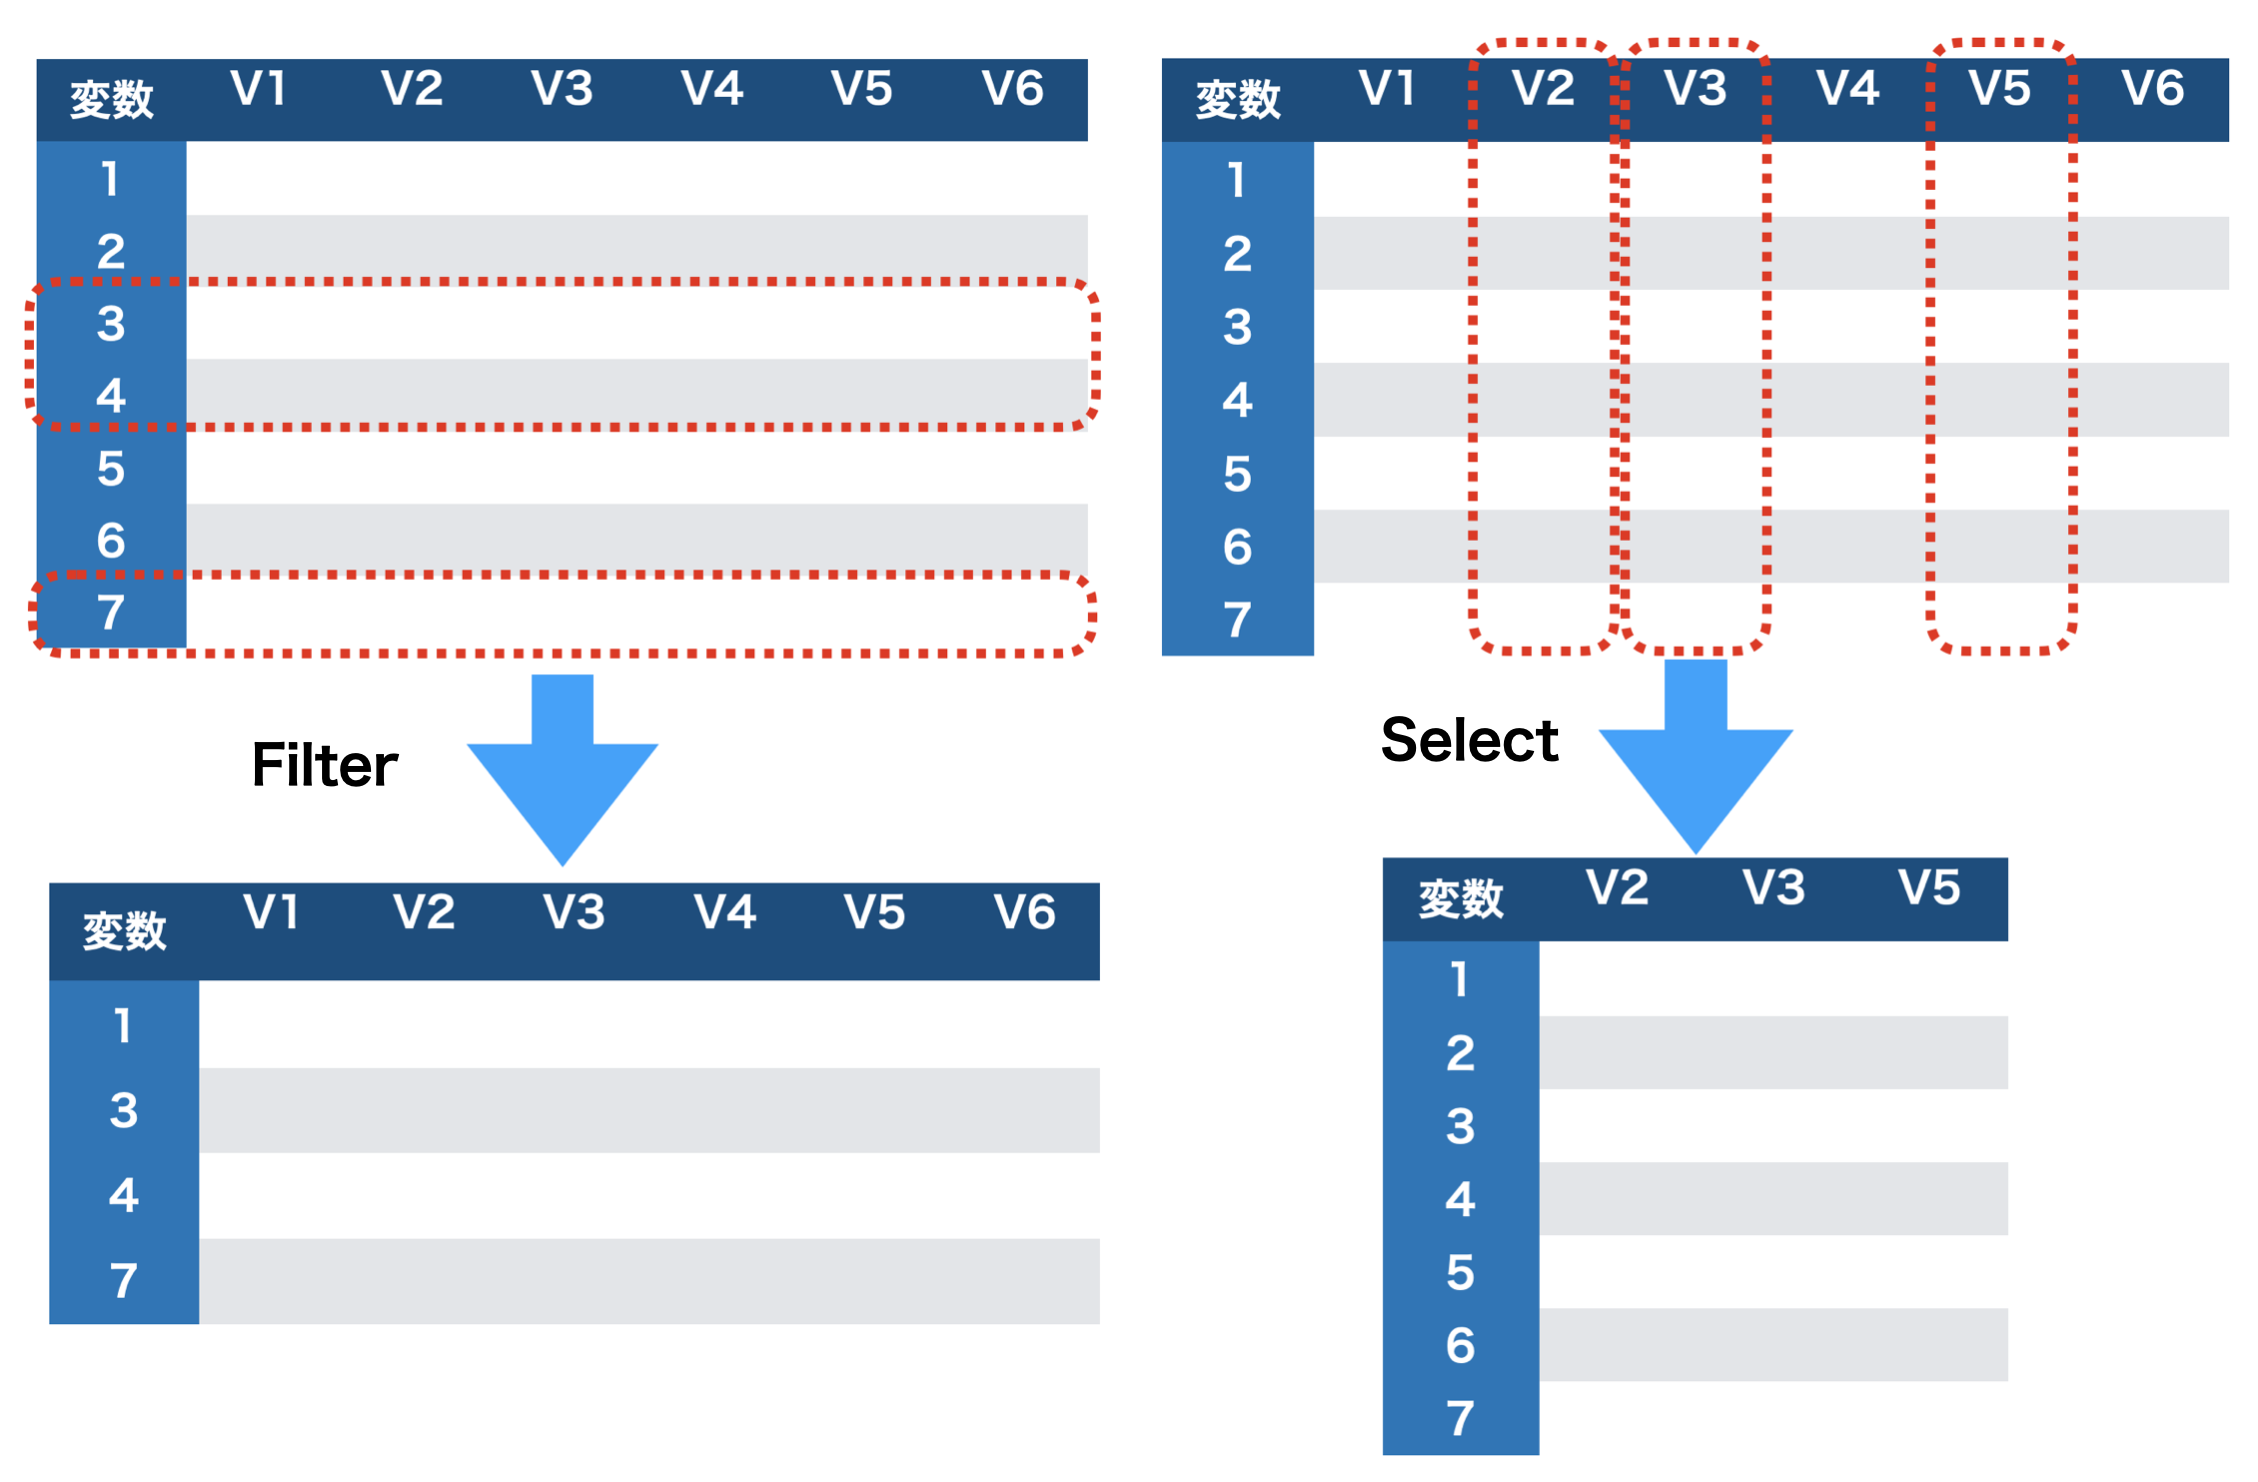
\includegraphics[keepaspectratio,width=0.8\linewidth]{figures/05_descriptives/filter_select.png}
	\caption{\texttt{filter}(左)と\texttt{select}(右)の違い}
	\label{fig:05_08}
\end{figure}

\paragraph{変数生成；mutate}
今度は変数を作る，mutateという関数です。たとえば打率は安打数を打席数で割ったもの，です。
今回のデータセットには安打数\verb|Hit|と打席数\verb|AtBats|はありますが，打率のデータがありません。これを作ろう，というときはコード\ref{code:usingR_mutate}のようにします。
\begin{lstlisting}[language=c++,label={code:usingR_mutate},caption={mutate関数}]
dat %>% select(AtBats,Hit) %>% mutate(BattingAverage = Hit / AtBats)
\end{lstlisting}
今回はいったん変数を選択してから，\verb|mutate|関数に入れました。もちろん直接入れてもらっても構いません。
いずれにせよ，これで変数が作れることがわかったと思います。

この「新しく変数を作る」というのは結構重要で，たとえばデータの中に欠測値があったとき，それを別の数字で置き換えるということがしたくなるかもしれません。\verb|mutate|関数で作る変数名を既存の変数名と同じにしておくと\textbf{上書き}されますから，これで書き換えることができます。

またデータサイエンスの実践上，変数同士の組み合わせからデータの特徴を表す別の変数を作り出したいということはよくあります。こうした加工のことを\keytermL{特徴量エンジニアリング}{とくちょうりょうえんじにありんぐ}といいます。

このように変数を加工することで，既存の変数から新しい変数をどんどん作っていくことができます。言い換えれば，データの加工はこれらの関数を使って，R上で記録を取りながら加工していきましょう，ということです。データを表計算ソフトで作っていて，そこで加工してしまうと\underline{データの捏造}が疑われる可能性があります。入力ミスや欠測値など不完全なデータであっても，それをどのように修正したかをすべてRで記録しながら進めていくことが，オープンサイエンスの取り組みとして重要なことなのです。入手したデータファイルは手を加えず，加工のプロセスをすべてオープンに明示しながら分析を進めていくことが重要です。

\end{document}
